\documentclass{article}
    % General document formatting
    \usepackage[margin=0.7in]{geometry}
    \usepackage[parfill]{parskip}
    \usepackage[utf8]{inputenc}
    
    % Related to math
    \usepackage{amsmath,amssymb,amsfonts,amsthm}
\usepackage{tikz}
\usepackage{subfigure}
\usetikzlibrary{bayesnet}

\begin{document}


\begin{figure}[ht]
\begin{center}
\begin{tabular}{cc}

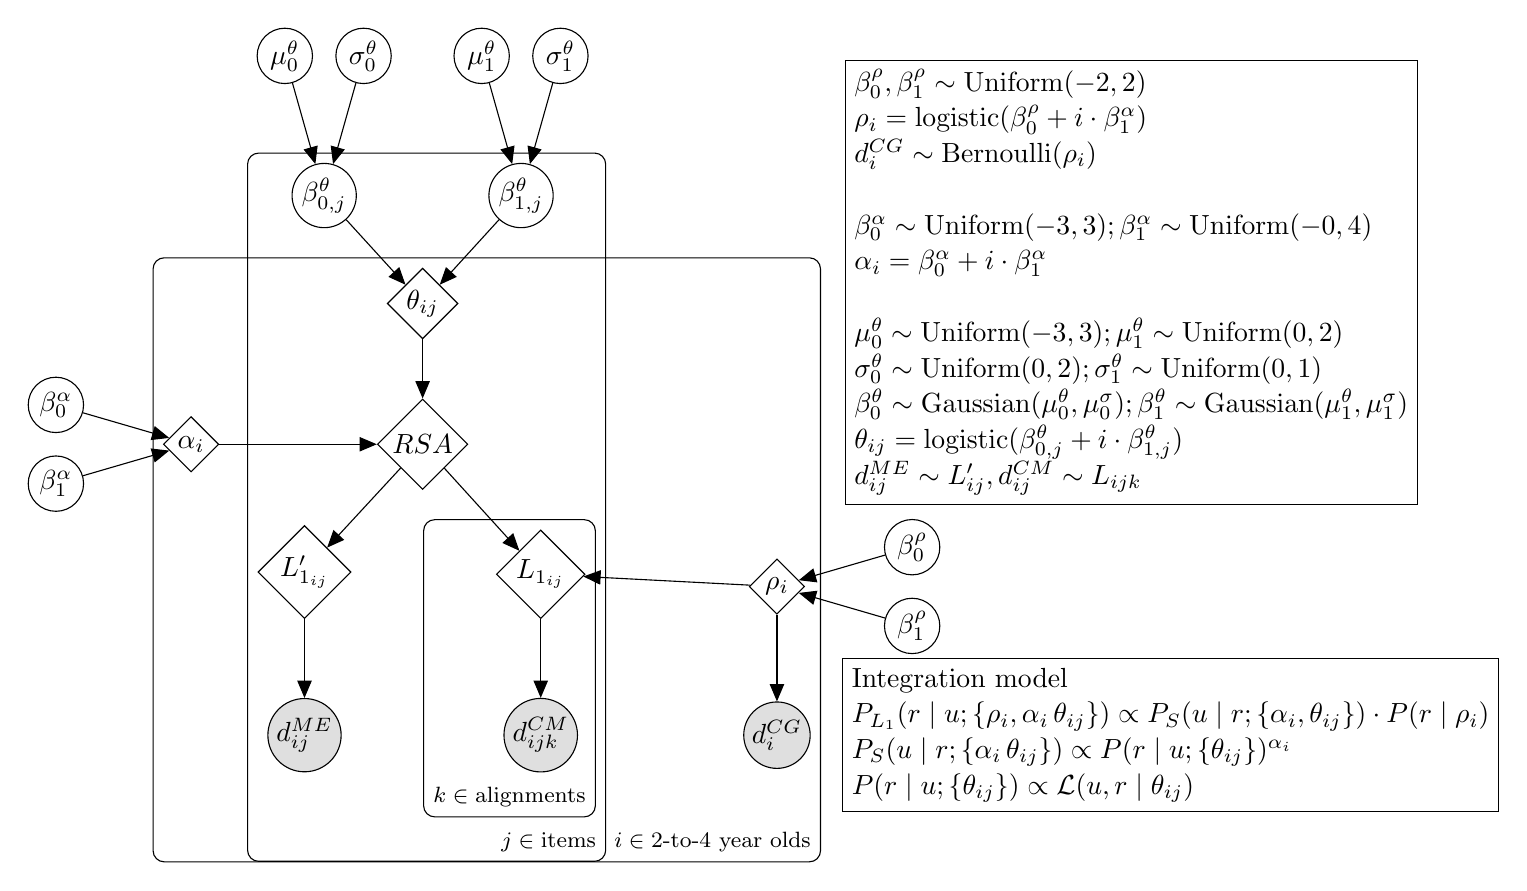
\begin{tikzpicture}
%% RSA nodes and data
\node[obs](data_comb){$d^{CM}_{ijk}$};
\node[obs, xshift=-3cm, yshift=0cm](data_me){$d^{ME}_{ij}$};
\node[obs, xshift=3cm,  yshift=0cm](data_cg){$d^{CG}_{i}$};

\node[det, above=of data_me](L1_me){$L'_{1_{ij}}$};
\node[det, above=of data_comb](L1_comb){$L_{1_{ij}}$};
\node[det, above=of L1_comb, xshift=-1.5cm, yshift=-0.5cm](RSA){$RSA$};

\edge{L1_me}{data_me};
\edge{L1_comb}{data_comb};
\edge{RSA}{L1_me};
\edge{RSA}{L1_comb};

% COMMON GROUND
\node[det, above=of data_cg, yshift=0.1cm](rho){$\rho_i$};
\node[latent, right=of rho, yshift=0.5cm](beta_rho_int){$\beta^{\rho}_0$};
\node[latent, right=of rho, yshift=-0.5cm](beta_rho_slope){$\beta^{\rho}_1$};

\edge{rho}{data_cg};
\edge{beta_rho_int}{rho};
\edge{beta_rho_slope}{rho};
\edge{rho}{L1_comb};

%% SPEAKER INFORMATIVITY

\node[det, left=of RSA, xshift=-1cm](alpha){$\alpha_i$};
\node[latent, left=of alpha, yshift=0.5cm](beta_alpha_int){$\beta^{\alpha}_0$};
\node[latent, left=of alpha, yshift=-0.5cm](beta_alpha_slope){$\beta^{\alpha}_1$};

%	\edge{alpha}{L1_me};
\edge{beta_alpha_int}{alpha};
\edge{beta_alpha_slope}{alpha};
\edge{alpha}{RSA};

%% SEMANTIC KNOWLEDGE model

	\node[det, above=of RSA, yshift=-0.25cm](theta){$\theta_{ij}$};
\node[latent, above=of theta, xshift=-1.25cm, yshift=-0.5cm](beta_theta_int){$\beta^{\theta}_{0, j}$};
\node[latent, above=of theta, xshift=1.25cm, yshift=-0.5cm](beta_theta_slope){$\beta^{\theta}_{1, j}$};

\node[latent, above=of beta_theta_int, xshift=-0.5cm](mu_theta_int){$\mu^{\theta}_{0}$};
\node[latent, above=of beta_theta_int, xshift=0.5cm](sigma_theta_int){$\sigma^{\theta}_{0}$};

\node[latent, above=of beta_theta_slope, xshift=-0.5cm](mu_theta_slope){$\mu^{\theta}_{1}$};
\node[latent, above=of beta_theta_slope, xshift=0.5cm](sigma_theta_slope){$\sigma^{\theta}_{1}$};

\edge{theta}{RSA};
%	\edge{theta}{L1_comb};
\edge{beta_theta_int}{theta};
\edge{beta_theta_slope}{theta};
\edge{mu_theta_int}{beta_theta_int};
\edge{sigma_theta_int}{beta_theta_int};
\edge{mu_theta_slope}{beta_theta_slope};
\edge{sigma_theta_slope}{beta_theta_slope};

\

\plate{plate_condition}{(data_comb)(L1_comb)}{$k \in \text{alignments}$};

	\plate{plate_items}{
%		(plate_data_me)
%		(plate_data_comb)
%		(plate_condition)
(plate_condition)
	(data_comb)
	(data_me)
	(L1_me)
	(L1_comb)
	(theta)
	(beta_theta_int)
	(beta_theta_slope)
}{$j \in \text{items}$}

	\plate{plate_data_comb}{
	(data_comb)
	(data_cg)
	(data_me)
	(plate_condition)
	(rho)
	(theta)
	(alpha)
	(L1_me)
	(L1_comb)
%		(plate_items)
	}{$i \in \text{2-to-4 year olds}$}



\node[draw, align=left, execute at begin node=\setlength{\baselineskip}{3ex}] at (7.5,5.75) { 
$\beta^\rho_0 ,\beta^\rho_1 \sim \text{Uniform}(-2,2)$ \\
 $\rho_i = \text{logistic}(\beta^\rho_0  + i \cdot \beta^\alpha_1)$ \\
 $d^{CG}_{i} \sim \text{Bernoulli}(\rho_i)$ \\
 \\
$\beta^\alpha_0 \sim \text{Uniform}(-3,3); \beta^\alpha_1 \sim \text{Uniform}(-0,4)$ \\
 $\alpha_i = \beta^\alpha_0  + i \cdot \beta^\alpha_1$ \\
 \\
 $\mu^\theta_0 \sim \text{Uniform}(-3,3); \mu^\theta_1 \sim \text{Uniform}(0,2)$ \\
 $\sigma^\theta_0 \sim \text{Uniform}(0,2); \sigma^\theta_1 \sim \text{Uniform}(0,1)$ \\
 $\beta^\theta_0 \sim \text{Gaussian}(\mu^\theta_0, \mu^\sigma_0); \beta^\theta_1 \sim \text{Gaussian}(\mu^\theta_1, \mu^\sigma_1)$  \\
 $\theta_{ij} = \text{logistic}(\beta^\theta_{0,j}  + i \cdot \beta^\theta_{1,j})$ \\
 $d^{ME}_{ij} \sim L'_{ij},  d^{CM}_{ij} \sim L_{ijk}$
};

\node[draw, align=left, execute at begin node=\setlength{\baselineskip}{3ex}] at (8,0) {Integration model\\ $P_{L_{1}}(r \mid u; \{\rho_i, \alpha_i\, \theta_{ij}\})\propto P_{S}(u \mid r; \{\alpha_i, \theta_{ij}\}) \cdot P(r \mid \rho_i) $\\ 
$P_{S}(u \mid r; \{\alpha_i\, \theta_{ij}\})\propto P(r \mid u; \{\theta_{ij}\}) ^{\alpha_i} $\\
$P(r \mid u; \{\theta_{ij}\}) \propto \mathcal{L}(u, r \mid \theta_{ij})$
};


\end{tikzpicture}


    \end{tabular}
  \end{center}
\end{figure}





\end{document}

